\subsection{Pengujian Komponen \textit{Resource Controller}}

Pada bagian ini akan dijelaskan tentang tujuan, skenario, hasil, dan analisis dari pengujian komponen \textbf{\textit{Resource Controller}}.

\subsubsection{Tujuan Pengujian}

Tujuan pengujian ini memastikan komponen \textbf{\textit{Resource Controller}} dapat berjalan dengan baik dan menghasilkan data yang sesuai dengan ekspektasi.

\subsubsection{Skenario Pengujian}

\textbf{\textit{Resource Controller}} adalah komponen \textit{low-level} yang hanya akan digunakan oleh komponen lain. Sehingga, untuk melakukan pengujian ini, akan dilakukan dengan pendekatan pembuatan \textit{test driver} khusus, program pengujian dapat dilihat pada gambar \ref{fig:rc-driver}. Pengujian terhadap komponen \textbf{\textit{Resource Controller}} dilakukan dengan beberapa skenario sebagai berikut.
\begin{enumerate}
    \item Mengubah alokasi prosesor maupun memori.
    \item Memastikan sistem antrian pengubahan alokasi berjalan dengan benar.
\end{enumerate}

\subsubsection{Hasil Pengujian dan Analisis}

Pada program pengujian yang dapat dilihat pada gambar \ref{fig:rc-driver}, pertama-tama akan ditambahkan memori sebesar 500MiB, dilanjutkan dengan menambah prosesor sejumlah 500m, kemudian, 1000m dan 1000MiB untuk prosesor dan memori, lalu terakhir, dikurangi sebesar 750m dan 1250MiB. Sebelum diubah, \textit{pods} memiliki konfigurasi yang dapat dilihat pada gambar \ref{fig:rc-state-0}. Untuk hasil pengubahan dapat dilihat pada gambar \ref{fig:rc-state-1}, \ref{fig:rc-state-2}, \ref{fig:rc-state-3}, dan \ref{fig:rc-state-4}. Kemudian program dijalankan ulang untuk melihat antrian pengubahan alokasi, gambar hasil pengujian dapat dilihat pada \ref{fig:rc-queue}. Dari pengujian tersebut, komponen sudah menjalankan tugas sesuai ekspektasi.

\begin{figure}[h]
    \centering
    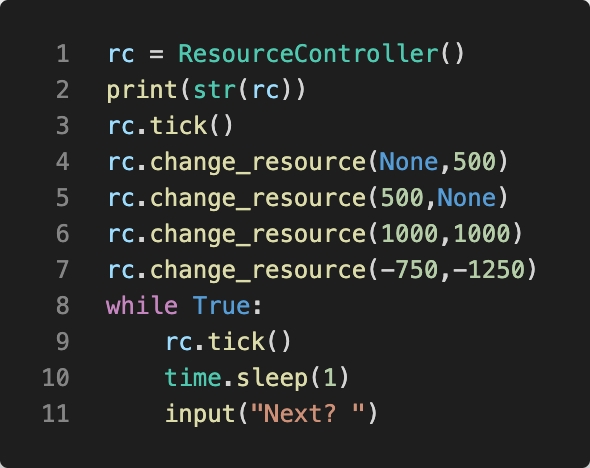
\includegraphics[width=0.8\textwidth]{chapter-4/rc-driver.png}
    \caption{Program \textit{Test Driver} untuk Menguji \textit{Resource Controller}}
    \label{fig:rc-driver}
\end{figure}

\begin{figure}[h]
    \centering
    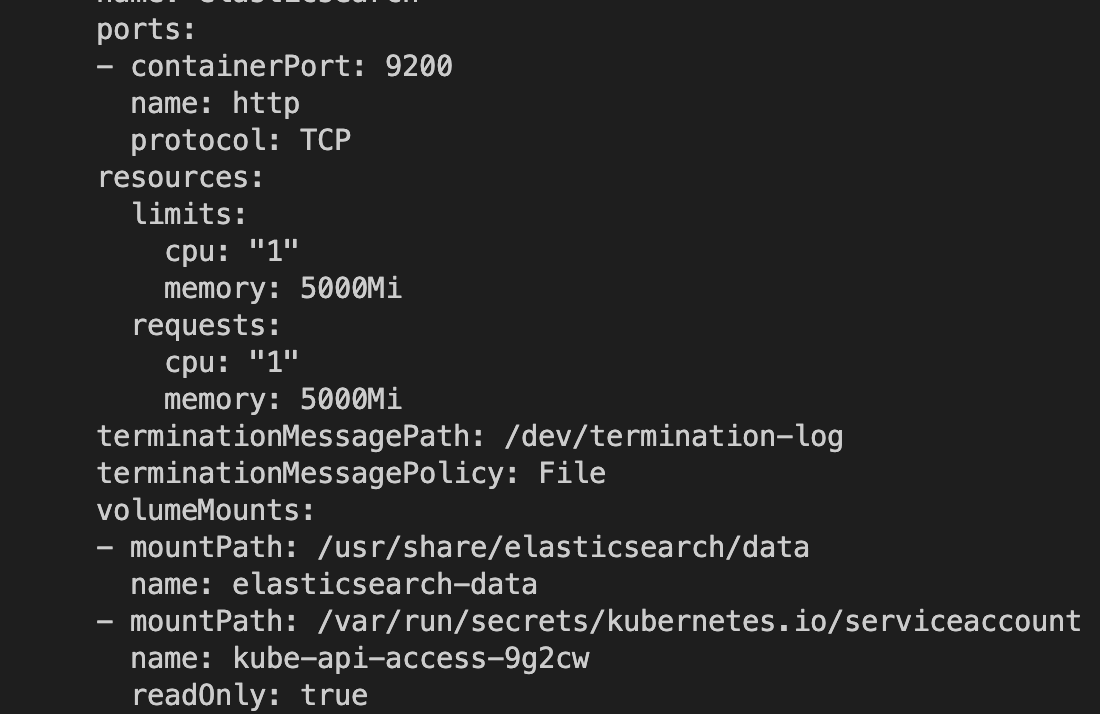
\includegraphics[width=0.8\textwidth]{chapter-4/rc-state-0.png}
    \caption{Status \textit{Pods} Sebelum Pengubahan Alokasi}
    \label{fig:rc-state-0}
\end{figure}

\begin{figure}[h]
    \centering
    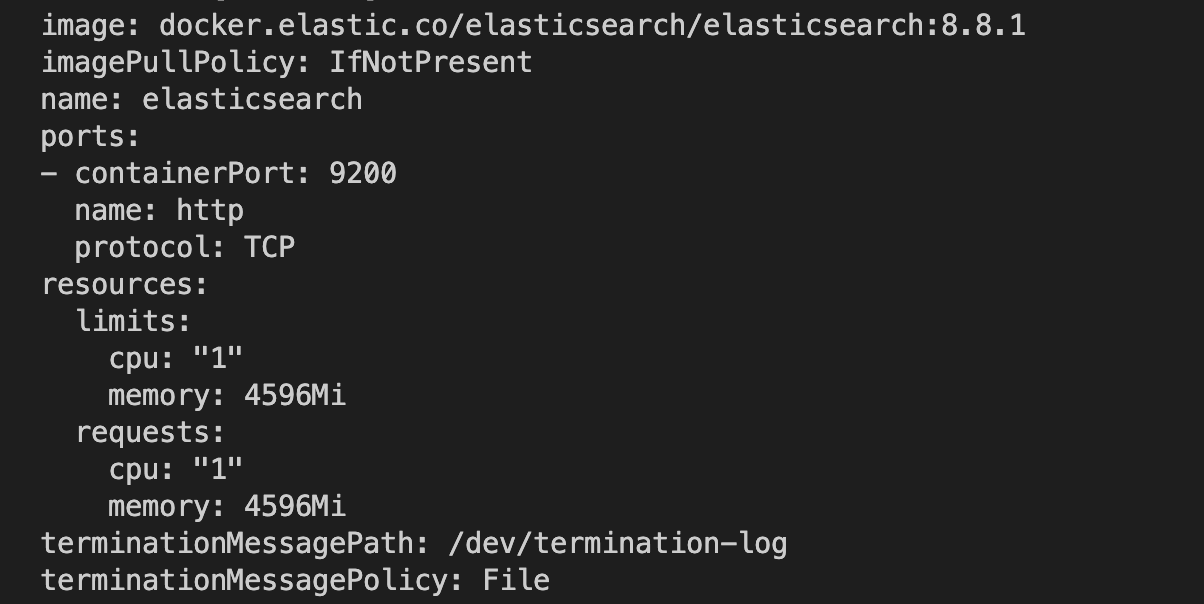
\includegraphics[width=0.8\textwidth]{chapter-4/rc-state-1.png}
    \caption{Status \textit{Pods} Setelah Pengubahan Pertama}
    \label{fig:rc-state-1}
\end{figure}

\begin{figure}[h]
    \centering
    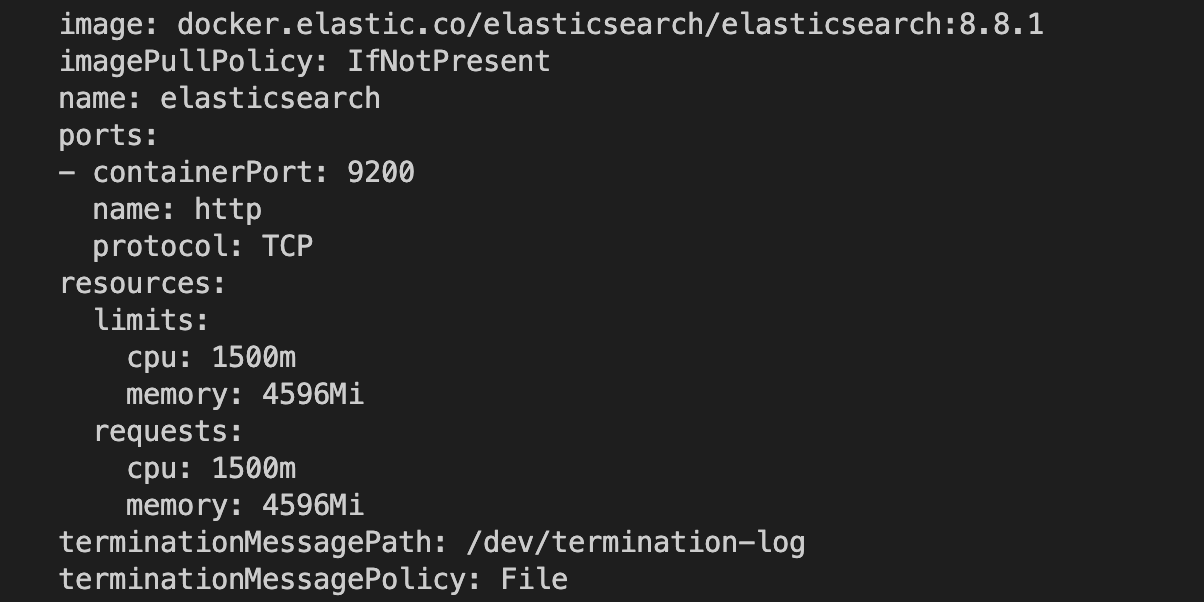
\includegraphics[width=0.8\textwidth]{chapter-4/rc-state-2.png}
    \caption{Status \textit{Pods} Setelah Pengubahan Kedua}
    \label{fig:rc-state-2}
\end{figure}

\begin{figure}[h]
    \centering
    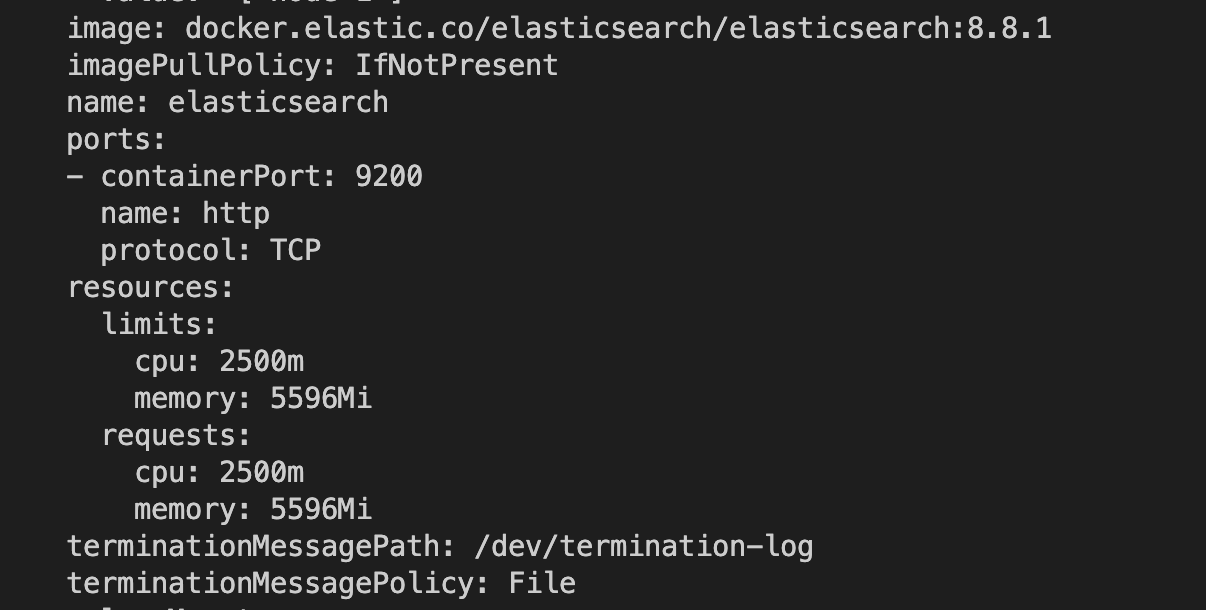
\includegraphics[width=0.8\textwidth]{chapter-4/rc-state-3.png}
    \caption{Status \textit{Pods} Setelah Pengubahan Ketiga}
    \label{fig:rc-state-3}
\end{figure}

\begin{figure}[h]
    \centering
    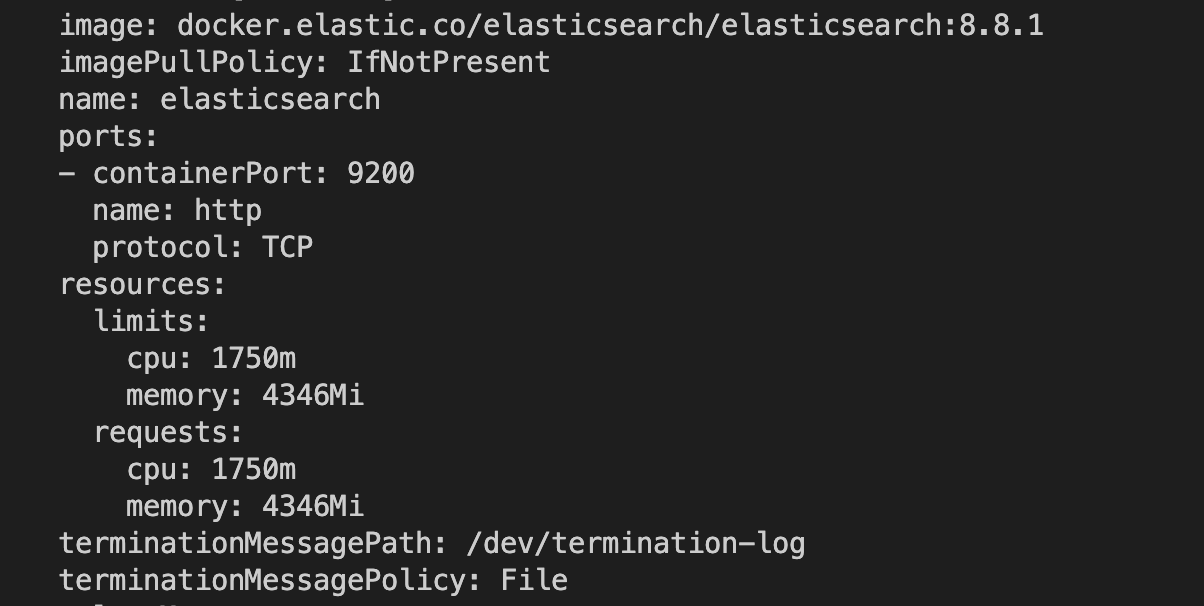
\includegraphics[width=0.8\textwidth]{chapter-4/rc-state-4.png}
    \caption{Status \textit{Pods} Setelah Pengubahan Keempat}
    \label{fig:rc-state-4}
\end{figure}

\begin{figure}[h]
    \centering
    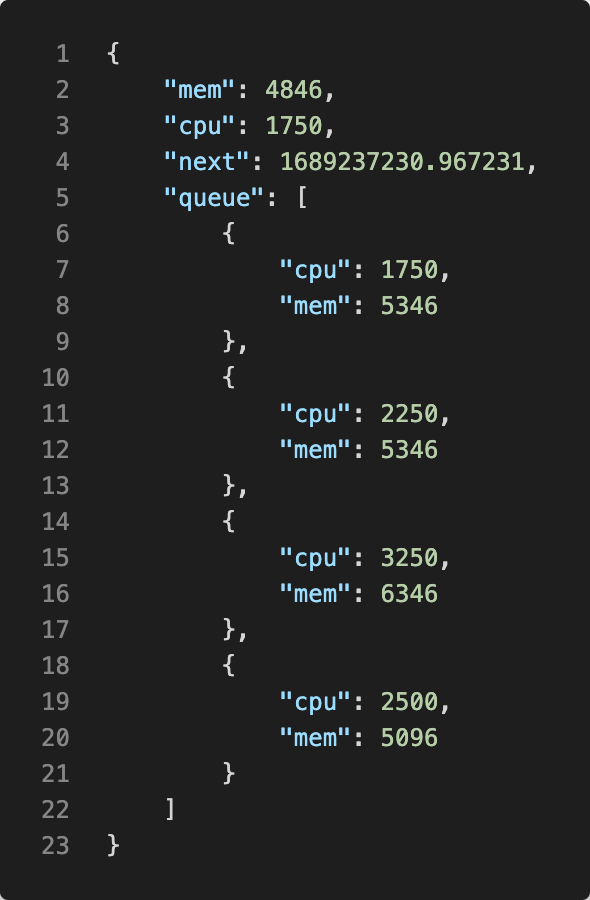
\includegraphics[width=0.8\textwidth]{chapter-4/rc-queue.png}
    \caption{Antrian Pengubahan Alokasi}
    \label{fig:rc-queue}
\end{figure}

Pengujian komponen \textbf{\textit{Resource Controller}} sudah sesuai ekspektasi dan dapat dilanjutkan ke pengujian komponen lainnya.